\documentclass[twoside]{book}

% Packages required by doxygen
\usepackage{fixltx2e}
\usepackage{calc}
\usepackage{doxygen}
\usepackage[export]{adjustbox} % also loads graphicx
\usepackage{graphicx}
\usepackage[utf8]{inputenc}
\usepackage{makeidx}
\usepackage{multicol}
\usepackage{multirow}
\PassOptionsToPackage{warn}{textcomp}
\usepackage{textcomp}
\usepackage[nointegrals]{wasysym}
\usepackage[table]{xcolor}

% Font selection
\usepackage[T1]{fontenc}
\usepackage[scaled=.90]{helvet}
\usepackage{courier}
\usepackage{amssymb}
\usepackage{sectsty}
\renewcommand{\familydefault}{\sfdefault}
\allsectionsfont{%
  \fontseries{bc}\selectfont%
  \color{darkgray}%
}
\renewcommand{\DoxyLabelFont}{%
  \fontseries{bc}\selectfont%
  \color{darkgray}%
}
\newcommand{\+}{\discretionary{\mbox{\scriptsize$\hookleftarrow$}}{}{}}

% Page & text layout
\usepackage{geometry}
\geometry{%
  a4paper,%
  top=2.5cm,%
  bottom=2.5cm,%
  left=2.5cm,%
  right=2.5cm%
}
\tolerance=750
\hfuzz=15pt
\hbadness=750
\setlength{\emergencystretch}{15pt}
\setlength{\parindent}{0cm}
\setlength{\parskip}{3ex plus 2ex minus 2ex}
\makeatletter
\renewcommand{\paragraph}{%
  \@startsection{paragraph}{4}{0ex}{-1.0ex}{1.0ex}{%
    \normalfont\normalsize\bfseries\SS@parafont%
  }%
}
\renewcommand{\subparagraph}{%
  \@startsection{subparagraph}{5}{0ex}{-1.0ex}{1.0ex}{%
    \normalfont\normalsize\bfseries\SS@subparafont%
  }%
}
\makeatother

% Headers & footers
\usepackage{fancyhdr}
\pagestyle{fancyplain}
\fancyhead[LE]{\fancyplain{}{\bfseries\thepage}}
\fancyhead[CE]{\fancyplain{}{}}
\fancyhead[RE]{\fancyplain{}{\bfseries\leftmark}}
\fancyhead[LO]{\fancyplain{}{\bfseries\rightmark}}
\fancyhead[CO]{\fancyplain{}{}}
\fancyhead[RO]{\fancyplain{}{\bfseries\thepage}}
\fancyfoot[LE]{\fancyplain{}{}}
\fancyfoot[CE]{\fancyplain{}{}}
\fancyfoot[RE]{\fancyplain{}{\bfseries\scriptsize Generated by Doxygen }}
\fancyfoot[LO]{\fancyplain{}{\bfseries\scriptsize Generated by Doxygen }}
\fancyfoot[CO]{\fancyplain{}{}}
\fancyfoot[RO]{\fancyplain{}{}}
\renewcommand{\footrulewidth}{0.4pt}
\renewcommand{\chaptermark}[1]{%
  \markboth{#1}{}%
}
\renewcommand{\sectionmark}[1]{%
  \markright{\thesection\ #1}%
}

% Indices & bibliography
\usepackage{natbib}
\usepackage[titles]{tocloft}
\setcounter{tocdepth}{3}
\setcounter{secnumdepth}{5}
\makeindex

% Custom commands
\newcommand{\clearemptydoublepage}{%
  \newpage{\pagestyle{empty}\cleardoublepage}%
}

\usepackage{caption}
\captionsetup{labelsep=space,justification=centering,font={bf},singlelinecheck=off,skip=4pt,position=top}

%===== C O N T E N T S =====

\begin{document}

% Titlepage & ToC
\pagenumbering{roman}
\begin{titlepage}
\vspace*{7cm}
\begin{center}%
{\Large Fire \& Ice \\[1ex]\large 1 }\\
\vspace*{1cm}
{\large Generated by Doxygen 1.8.11}\\
\end{center}
\end{titlepage}
\clearemptydoublepage
\tableofcontents
\clearemptydoublepage
\pagenumbering{arabic}

%--- Begin generated contents ---
\chapter{Hierarchical Index}
\section{Class Hierarchy}
This inheritance list is sorted roughly, but not completely, alphabetically\+:\begin{DoxyCompactList}
\item \contentsline{section}{Animation}{\pageref{classAnimation}}{}
\item \contentsline{section}{Client}{\pageref{classClient}}{}
\item \contentsline{section}{Game}{\pageref{classGame}}{}
\item \contentsline{section}{Obj\+Man\+:\+:Game\+Obj\+Dealloc}{\pageref{structObjMan_1_1GameObjDealloc}}{}
\item \contentsline{section}{Game\+State}{\pageref{classGameState}}{}
\item \contentsline{section}{Level\+Menu}{\pageref{classLevelMenu}}{}
\item \contentsline{section}{Main\+Menu}{\pageref{classMainMenu}}{}
\item \contentsline{section}{Obj\+Man}{\pageref{classObjMan}}{}
\item \contentsline{section}{Server}{\pageref{classServer}}{}
\item \contentsline{section}{Splash}{\pageref{classSplash}}{}
\item \contentsline{section}{Visible\+Game\+Object}{\pageref{classVisibleGameObject}}{}
\begin{DoxyCompactList}
\item \contentsline{section}{Platform}{\pageref{classPlatform}}{}
\item \contentsline{section}{Player}{\pageref{classPlayer}}{}
\end{DoxyCompactList}
\end{DoxyCompactList}

\chapter{Data Structure Index}
\section{Data Structures}
Here are the data structures with brief descriptions\+:\begin{DoxyCompactList}
\item\contentsline{section}{{\bf Animation} }{\pageref{classAnimation}}{}
\item\contentsline{section}{{\bf Client} \\*Stores info reg. the connection with another \char`\"{}server\char`\"{} }{\pageref{classClient}}{}
\item\contentsline{section}{{\bf Game} \\*Saves the current state of the game }{\pageref{classGame}}{}
\item\contentsline{section}{{\bf Obj\+Man\+::\+Game\+Obj\+Dealloc} \\*A functor for deallocating the memory given to each \doxyref{Visible\+Game\+Object}{p.}{classVisibleGameObject} }{\pageref{structObjMan_1_1GameObjDealloc}}{}
\item\contentsline{section}{{\bf Game\+State} }{\pageref{classGameState}}{}
\item\contentsline{section}{{\bf Level\+Menu} \\*This is a level menu object }{\pageref{classLevelMenu}}{}
\item\contentsline{section}{{\bf Main\+Menu} \\*This is a main menu object }{\pageref{classMainMenu}}{}
\item\contentsline{section}{{\bf Obj\+Man} \\*A drawable object manager }{\pageref{classObjMan}}{}
\item\contentsline{section}{{\bf Platform} \\*This class stores any objects that are not \char`\"{}players\char`\"{} for now. New classes for each object can be added later. Objects are differentiated by their \char`\"{}texture filename\char`\"{} }{\pageref{classPlatform}}{}
\item\contentsline{section}{{\bf Player} \\*Updates and checks Collision of Fire\+Boy/\+Water\+Girl with various objects }{\pageref{classPlayer}}{}
\item\contentsline{section}{{\bf Server} \\*A server over T\+CP to enable networking }{\pageref{classServer}}{}
\item\contentsline{section}{{\bf Splash} \\*Saves \doxyref{Game}{p.}{classGame} state }{\pageref{classSplash}}{}
\item\contentsline{section}{{\bf Visible\+Game\+Object} \\*This class is used to define an object that is to be drawn on the screen }{\pageref{classVisibleGameObject}}{}
\end{DoxyCompactList}

\chapter{Data Structure Documentation}
\section{Animation Class Reference}
\label{classAnimation}\index{Animation@{Animation}}
\subsection*{Public Member Functions}
\begin{DoxyCompactItemize}
\item 
void {\bf update} (int row, float delta\+Time, bool face\+Right)
\begin{DoxyCompactList}\small\item\em Takes the row from the compound texture. \end{DoxyCompactList}\item 
void {\bf create} (sf\+::\+Texture $\ast$texture, sf\+::\+Vector2u {\bf image\+Count}, float switch\+Time)
\begin{DoxyCompactList}\small\item\em Creates the animation. \end{DoxyCompactList}\end{DoxyCompactItemize}
\subsection*{Data Fields}
\begin{DoxyCompactItemize}
\item 
sf\+::\+Int\+Rect {\bf uv\+Rect}\label{classAnimation_a82c41dd15d9a98ecc0699ecca09fd056}

\begin{DoxyCompactList}\small\item\em Accounts for cropping 1 image out of the entire compound image. \end{DoxyCompactList}\end{DoxyCompactItemize}
\subsection*{Private Attributes}
\begin{DoxyCompactItemize}
\item 
sf\+::\+Vector2u {\bf image\+Count}\label{classAnimation_ae4bc32c6c921bd2161350152ce12e09c}

\begin{DoxyCompactList}\small\item\em Vector which gives a count of the total images in compund image file. \end{DoxyCompactList}\item 
sf\+::\+Vector2u {\bf current\+Image}\label{classAnimation_aeb23dec031861eff3dda1b759f4472fc}

\begin{DoxyCompactList}\small\item\em The image point at which the animation row is running at the moment. \end{DoxyCompactList}\item 
float {\bfseries total\+Time}\label{classAnimation_a04f09b9faedd40c52a9b60b800e10ea8}

\item 
float {\bfseries switch\+Time}\label{classAnimation_a7b2fb4577ab94e863b88ec6cf96cc8b6}

\end{DoxyCompactItemize}


\subsection{Detailed Description}


Definition at line 5 of file Animation.\+h.



\subsection{Member Function Documentation}
\index{Animation@{Animation}!create@{create}}
\index{create@{create}!Animation@{Animation}}
\subsubsection[{create(sf\+::\+Texture $\ast$texture, sf\+::\+Vector2u image\+Count, float switch\+Time)}]{\setlength{\rightskip}{0pt plus 5cm}void Animation\+::create (
\begin{DoxyParamCaption}
\item[{sf\+::\+Texture $\ast$}]{texture, }
\item[{sf\+::\+Vector2u}]{image\+Count, }
\item[{float}]{switch\+Time}
\end{DoxyParamCaption}
)}\label{classAnimation_a2597dbf92eb582f4610abee8a9e2aaeb}


Creates the animation. 


\begin{DoxyParams}{Parameters}
{\em texture} & \\
\hline
{\em image\+Count} & \\
\hline
{\em switch\+Time} & Takes the imagecount , switchtime and texture as parameters and updates the correspponding private member variables. \\
\hline
\end{DoxyParams}
\index{Animation@{Animation}!update@{update}}
\index{update@{update}!Animation@{Animation}}
\subsubsection[{update(int row, float delta\+Time, bool face\+Right)}]{\setlength{\rightskip}{0pt plus 5cm}void Animation\+::update (
\begin{DoxyParamCaption}
\item[{int}]{row, }
\item[{float}]{delta\+Time, }
\item[{bool}]{face\+Right}
\end{DoxyParamCaption}
)}\label{classAnimation_af09462caccc4d41ebfe288f703c4facd}


Takes the row from the compound texture. 


\begin{DoxyParams}{Parameters}
{\em row} & \\
\hline
{\em delta\+Time} & \\
\hline
{\em face\+Right} & Row is taken as input from the source image and sets animation by running through the row. Delta\+Time counts for the animation switch time. Face\+Right is used for checking the direction of movement of player for loading texture. \\
\hline
\end{DoxyParams}


The documentation for this class was generated from the following file\+:\begin{DoxyCompactItemize}
\item 
Animation.\+h\end{DoxyCompactItemize}

\section{Client Class Reference}
\label{classClient}\index{Client@{Client}}


Stores info reg. the connection with another \char`\"{}server\char`\"{}.  




{\ttfamily \#include $<$Client.\+h$>$}

\subsection*{Public Member Functions}
\begin{DoxyCompactItemize}
\item 
{\bf Client} ()=default\label{classClient_ac13ad1e98c47db57ce0823dc735261cd}

\begin{DoxyCompactList}\small\item\em The default constructor. \end{DoxyCompactList}\end{DoxyCompactItemize}
\subsection*{Data Fields}
\begin{DoxyCompactItemize}
\item 
sf\+::\+Tcp\+Socket {\bf send\+Socket}\label{classClient_a08b3297842eb2b464d275ef591f9cc73}

\begin{DoxyCompactList}\small\item\em Tcp\+Socket used by client to send info to the server. \end{DoxyCompactList}\item 
sf\+::\+Tcp\+Socket {\bf listen\+Socket}\label{classClient_a09b45ef7a1057f3d3fbb38be8bb46db1}

\begin{DoxyCompactList}\small\item\em Tcp\+Socket used by client to receive info from the server. \end{DoxyCompactList}\end{DoxyCompactItemize}


\subsection{Detailed Description}
Stores info reg. the connection with another \char`\"{}server\char`\"{}. 

Definition at line 13 of file Client.\+h.



The documentation for this class was generated from the following file\+:\begin{DoxyCompactItemize}
\item 
Client.\+h\end{DoxyCompactItemize}

\section{Game Class Reference}
\label{classGame}\index{Game@{Game}}


Saves the current state of the game.  




\subsection{Detailed Description}
Saves the current state of the game. 

Saves the state similar to a finite state machine transitioning between various states which define the snapshot of game at any instant. Some of the states include game in Playing State , At Main Menu or the server waiting for its client.

Takes the responsibility of setting up the server and keeping it\textquotesingle{}s state in sync with it\textquotesingle{}s client.

All the members of the class are static as the class is not instantiated and require to set up with an intialiser list.

Pushes the state to Waitfor\+Client if client calls for joining and to Waitfor\+Server if process wishes to create a server. 

The documentation for this class was generated from the following file\+:\begin{DoxyCompactItemize}
\item 
Game\+State.\+h\end{DoxyCompactItemize}

\section{Obj\+Man\+:\+:Game\+Obj\+Dealloc Struct Reference}
\label{structObjMan_1_1GameObjDealloc}\index{Obj\+Man\+::\+Game\+Obj\+Dealloc@{Obj\+Man\+::\+Game\+Obj\+Dealloc}}


A functor for deallocating the memory given to each \doxyref{Visible\+Game\+Object}{p.}{classVisibleGameObject}.  


\subsection*{Public Member Functions}
\begin{DoxyCompactItemize}
\item 
void {\bfseries operator()} (const std\+::pair$<$ std\+::string, {\bf Visible\+Game\+Object} $\ast$ $>$ \&a) const \label{structObjMan_1_1GameObjDealloc_a24f7d3afb3e9bad6d17016ced5469817}

\end{DoxyCompactItemize}


\subsection{Detailed Description}
A functor for deallocating the memory given to each \doxyref{Visible\+Game\+Object}{p.}{classVisibleGameObject}. 

Definition at line 80 of file Obj\+Man.\+h.



The documentation for this struct was generated from the following file\+:\begin{DoxyCompactItemize}
\item 
Obj\+Man.\+h\end{DoxyCompactItemize}

\section{Game\+State Class Reference}
\label{classGameState}\index{Game\+State@{Game\+State}}
\subsection*{Public Types}
\begin{DoxyCompactItemize}
\item 
enum {\bf state} \{ \\*
{\bf Not\+\_\+init}, 
{\bf Level\+Check}, 
{\bf At\+Splash}, 
{\bf At\+Menu}, 
\\*
{\bf Wait\+For\+Client}, 
{\bf Wait\+For\+Server}, 
{\bf Playing}, 
{\bf Exiting}, 
\\*
{\bf Game\+Over}, 
{\bfseries Game\+Won}
 \}
\end{DoxyCompactItemize}
\subsection*{Static Public Member Functions}
\begin{DoxyCompactItemize}
\item 
static void {\bf play} ()
\begin{DoxyCompactList}\small\item\em Start Playing the game! \end{DoxyCompactList}\item 
static void {\bf Load\+From\+File} (unsigned int level)
\begin{DoxyCompactList}\small\item\em Has the task of loading the resources from the Level$<$num$>$.\+text file which sets up the required resources for setting up the level. \end{DoxyCompactList}\end{DoxyCompactItemize}
\subsection*{Static Public Attributes}
\begin{DoxyCompactItemize}
\item 
static bool {\bf file\+Path}
\begin{DoxyCompactList}\small\item\em The way paths are written\+: false for linux, true for O\+SX. \end{DoxyCompactList}\item 
static const unsigned short {\bf \+\_\+resX} \{1600\}
\begin{DoxyCompactList}\small\item\em Horizontal Resolution. \end{DoxyCompactList}\item 
static const unsigned short {\bf \+\_\+resY} \{900\}
\begin{DoxyCompactList}\small\item\em Vertical Resolution. \end{DoxyCompactList}\item 
static {\bf state} {\bf \+\_\+state}\label{classGameState_afcf1225baf36dc7131c39e8c1b33e2df}

\begin{DoxyCompactList}\small\item\em Stores the current state of game. \end{DoxyCompactList}\item 
static {\bf Server} {\bf server}\label{classGameState_a5dca528501718f1ed4fa892b71db265a}

\begin{DoxyCompactList}\small\item\em Object representing the server class initialised in initiation list with the listening and sending ports. \end{DoxyCompactList}\item 
static {\bf Client} {\bf client}\label{classGameState_a7e631641790c7234bfd4555d6e29ced4}

\begin{DoxyCompactList}\small\item\em Oject representing the client class initialised in initiation list with the listening and sending ports. \end{DoxyCompactList}\item 
static bool {\bf is\+Client}\label{classGameState_ad2e7616dfd52a11dce956bee24a1fc24}

\begin{DoxyCompactList}\small\item\em A boolean which checks if the running code is exectued from client or server side. \end{DoxyCompactList}\item 
static unsigned short {\bf port1}\label{classGameState_a70fed938c1374c60303395ab7e5144c3}

\begin{DoxyCompactList}\small\item\em Represents sending port for server and listening for client. \end{DoxyCompactList}\item 
static unsigned short {\bf port2}\label{classGameState_aac02f0e00bdc1b7bc3977f7108d9c44b}

\begin{DoxyCompactList}\small\item\em Represents listening port for server and sending for client. \end{DoxyCompactList}\item 
static unsigned short {\bf \+\_\+cur\+Level}\label{classGameState_a0a00e7afe1ead236555bf58eae2b1e79}

\begin{DoxyCompactList}\small\item\em Integer variable to denote the state of current level. \end{DoxyCompactList}\item 
static std\+::mutex {\bf race}
\begin{DoxyCompactList}\small\item\em Race -\/ A mutex for keeping the state of switch. \end{DoxyCompactList}\item 
static std\+::vector$<$ {\bf Visible\+Game\+Object} $\ast$ $>$ {\bf \+\_\+obj\+To\+Be\+Acted}\label{classGameState_a987cc8791aabb50c45436ef811981b44}

\begin{DoxyCompactList}\small\item\em Contains the objects (switch) state , checks whether they are activated or not which leads to further change other objects. \end{DoxyCompactList}\item 
static unsigned short {\bf red\+Gems\+Collected}\label{classGameState_ae3f0b95917fbf8cf959d16b8c467617f}

\begin{DoxyCompactList}\small\item\em Contains the number of red gems collected by the fireboy . \end{DoxyCompactList}\item 
static unsigned short {\bf blue\+Gems\+Collected}\label{classGameState_ad7ff58b7e5663432ec3251a3850e89c7}

\begin{DoxyCompactList}\small\item\em Contains the number of blue gems collected by the watergirl . \end{DoxyCompactList}\item 
static unsigned short {\bf max\+Red\+Gems}\label{classGameState_a8b9ef12593d42d0ca118fce41e461901}

\begin{DoxyCompactList}\small\item\em \doxyref{Game}{p.}{classGame} completes if max\+Red\+Gems is equal to the Red gems collected. \end{DoxyCompactList}\item 
static unsigned short {\bf max\+Blue\+Gems}\label{classGameState_a20e403812b2dba7afc9e1ef5ee78e0b0}

\begin{DoxyCompactList}\small\item\em \doxyref{Game}{p.}{classGame} completes if max\+Blue\+Gems is equal to the Blue gems collected. \end{DoxyCompactList}\item 
static bool {\bf \+\_\+winI}\label{classGameState_ac1f9dd3ed1dd581f4e6af69fec6e497d}

\begin{DoxyCompactList}\small\item\em Boolean checks whether Ice door is opened or not. \end{DoxyCompactList}\item 
static bool {\bf \+\_\+winF}\label{classGameState_ac6ff35654e9d1b318dd9053619501764}

\begin{DoxyCompactList}\small\item\em Boolean checks whether Fire door is opened or not. \end{DoxyCompactList}\end{DoxyCompactItemize}
\subsection*{Static Private Member Functions}
\begin{DoxyCompactItemize}
\item 
static bool {\bf is\+Exiting} ()\label{classGameState_a9512f495df14d5351178e8a6ba291343}

\begin{DoxyCompactList}\small\item\em Check if the game is in Exiting state. \end{DoxyCompactList}\item 
static void {\bf game\+Loop} ()\label{classGameState_a0430d274df28d8c32cbf193156073c38}

\begin{DoxyCompactList}\small\item\em The big game loop which keeps the game going, checking for events. \end{DoxyCompactList}\item 
static void {\bf show\+Splash\+Screen} ()\label{classGameState_a265220f00d5a1ea797d2e23e3ba2a9a9}

\begin{DoxyCompactList}\small\item\em Init and show a splash screen. \end{DoxyCompactList}\item 
static void {\bf show\+Main\+Menu} ()\label{classGameState_ada212938e5b2116507f13cfb5ff4d406}

\begin{DoxyCompactList}\small\item\em Shows the Main menu , option to create or join server after flash screen. \end{DoxyCompactList}\item 
static void {\bf show\+Level\+Screen} ()\label{classGameState_a9acf57cfc15e7c3f2e347a5d06d08ac6}

\begin{DoxyCompactList}\small\item\em Shows the Level Screen , for selecting the level. \end{DoxyCompactList}\end{DoxyCompactItemize}
\subsection*{Static Private Attributes}
\begin{DoxyCompactItemize}
\item 
static {\bf Player} $\ast$ {\bf fireboy}
\begin{DoxyCompactList}\small\item\em The current state of the game. \end{DoxyCompactList}\item 
static {\bf Player} $\ast$ {\bf watergirl}
\begin{DoxyCompactList}\small\item\em \doxyref{Player}{p.}{classPlayer} from the client. \end{DoxyCompactList}\item 
static {\bf Obj\+Man} {\bf \+\_\+game\+Object\+Manager}
\begin{DoxyCompactList}\small\item\em Holds all the objects as a map. \end{DoxyCompactList}\item 
static sf\+::\+Render\+Window {\bf \+\_\+main\+Window}
\begin{DoxyCompactList}\small\item\em The main window. \end{DoxyCompactList}\end{DoxyCompactItemize}


\subsection{Detailed Description}


Definition at line 30 of file Game\+State.\+h.



\subsection{Member Enumeration Documentation}
\index{Game\+State@{Game\+State}!state@{state}}
\index{state@{state}!Game\+State@{Game\+State}}
\subsubsection[{state}]{\setlength{\rightskip}{0pt plus 5cm}enum {\bf Game\+State\+::state}}\label{classGameState_a097555f82a7b1dc23fee373b6a61cfd4}
\begin{Desc}
\item[Enumerator]\par
\begin{description}
\index{Not\+\_\+init@{Not\+\_\+init}!Game\+State@{Game\+State}}\index{Game\+State@{Game\+State}!Not\+\_\+init@{Not\+\_\+init}}\item[{\em 
Not\+\_\+init\label{classGameState_a097555f82a7b1dc23fee373b6a61cfd4a99098609fb37f1e88dd4d98a4f9bb5d7}
}]\doxyref{Game}{p.}{classGame} is not init. \index{Level\+Check@{Level\+Check}!Game\+State@{Game\+State}}\index{Game\+State@{Game\+State}!Level\+Check@{Level\+Check}}\item[{\em 
Level\+Check\label{classGameState_a097555f82a7b1dc23fee373b6a61cfd4a0059fdbafc3ababdc9cfa7eecba159c2}
}]Level Selection Menu. \index{At\+Splash@{At\+Splash}!Game\+State@{Game\+State}}\index{Game\+State@{Game\+State}!At\+Splash@{At\+Splash}}\item[{\em 
At\+Splash\label{classGameState_a097555f82a7b1dc23fee373b6a61cfd4aaa8e7a1b7d5956e0fb1ce7806fffe6fb}
}]\doxyref{Splash}{p.}{classSplash} state of \doxyref{Game}{p.}{classGame}. \index{At\+Menu@{At\+Menu}!Game\+State@{Game\+State}}\index{Game\+State@{Game\+State}!At\+Menu@{At\+Menu}}\item[{\em 
At\+Menu\label{classGameState_a097555f82a7b1dc23fee373b6a61cfd4adb178a8bdb06194fd46a2c85fe7caa41}
}]The main menu of game. \index{Wait\+For\+Client@{Wait\+For\+Client}!Game\+State@{Game\+State}}\index{Game\+State@{Game\+State}!Wait\+For\+Client@{Wait\+For\+Client}}\item[{\em 
Wait\+For\+Client\label{classGameState_a097555f82a7b1dc23fee373b6a61cfd4ae2ddbefa150f2b70bfc9fc64e0e46f40}
}]\doxyref{Server}{p.}{classServer} waiting state for \doxyref{Client}{p.}{classClient}. \index{Wait\+For\+Server@{Wait\+For\+Server}!Game\+State@{Game\+State}}\index{Game\+State@{Game\+State}!Wait\+For\+Server@{Wait\+For\+Server}}\item[{\em 
Wait\+For\+Server\label{classGameState_a097555f82a7b1dc23fee373b6a61cfd4a0bcbdd45b3b7fe99e26666ca9587f848}
}]\doxyref{Client}{p.}{classClient} waiting for \doxyref{Server}{p.}{classServer}. \index{Playing@{Playing}!Game\+State@{Game\+State}}\index{Game\+State@{Game\+State}!Playing@{Playing}}\item[{\em 
Playing\label{classGameState_a097555f82a7b1dc23fee373b6a61cfd4a0c7c919903ffb50f3d56b0ef11fb5532}
}]The right on playing state. \index{Exiting@{Exiting}!Game\+State@{Game\+State}}\index{Game\+State@{Game\+State}!Exiting@{Exiting}}\item[{\em 
Exiting\label{classGameState_a097555f82a7b1dc23fee373b6a61cfd4a68fe39f597c784cd2e6e2626bcbb897f}
}]Windowexits. \index{Game\+Over@{Game\+Over}!Game\+State@{Game\+State}}\index{Game\+State@{Game\+State}!Game\+Over@{Game\+Over}}\item[{\em 
Game\+Over\label{classGameState_a097555f82a7b1dc23fee373b6a61cfd4a822b1b51894f1d852fb6890e2220a574}
}]Shows the defeat of player. \end{description}
\end{Desc}


Definition at line 72 of file Game\+State.\+h.



\subsection{Member Function Documentation}
\index{Game\+State@{Game\+State}!Load\+From\+File@{Load\+From\+File}}
\index{Load\+From\+File@{Load\+From\+File}!Game\+State@{Game\+State}}
\subsubsection[{Load\+From\+File(unsigned int level)}]{\setlength{\rightskip}{0pt plus 5cm}static void Game\+State\+::\+Load\+From\+File (
\begin{DoxyParamCaption}
\item[{unsigned int}]{level}
\end{DoxyParamCaption}
)\hspace{0.3cm}{\ttfamily [static]}}\label{classGameState_a99bb89bb694d8e686a24c30557c1ad2a}


Has the task of loading the resources from the Level$<$num$>$.\+text file which sets up the required resources for setting up the level. 

Reserves memory in heap for all the Game\+Objects and adds them into a map as a common storage entity. 
\begin{DoxyParams}{Parameters}
{\em level} & \\
\hline
\end{DoxyParams}
\index{Game\+State@{Game\+State}!play@{play}}
\index{play@{play}!Game\+State@{Game\+State}}
\subsubsection[{play()}]{\setlength{\rightskip}{0pt plus 5cm}static void Game\+State\+::play (
\begin{DoxyParamCaption}
{}
\end{DoxyParamCaption}
)\hspace{0.3cm}{\ttfamily [static]}}\label{classGameState_a475c2829f28c61363c540316a591d372}


Start Playing the game! 

Sets the game running up right on and loads all the required resources (fonts or images) . Renders the main window and pushes the game to the \doxyref{Splash}{p.}{classSplash} flashing state and sets up the main \doxyref{Game}{p.}{classGame} Loop in action 

\subsection{Field Documentation}
\index{Game\+State@{Game\+State}!\+\_\+game\+Object\+Manager@{\+\_\+game\+Object\+Manager}}
\index{\+\_\+game\+Object\+Manager@{\+\_\+game\+Object\+Manager}!Game\+State@{Game\+State}}
\subsubsection[{\+\_\+game\+Object\+Manager}]{\setlength{\rightskip}{0pt plus 5cm}{\bf Obj\+Man} Game\+State\+::\+\_\+game\+Object\+Manager\hspace{0.3cm}{\ttfamily [static]}, {\ttfamily [private]}}\label{classGameState_a31259a9b548fd1d5dbe02da361a94b4c}


Holds all the objects as a map. 

A class which has the responsibility of keeping all the game objects in a container , a map in this case iteration over which is used to update every object. 

Definition at line 193 of file Game\+State.\+h.

\index{Game\+State@{Game\+State}!\+\_\+main\+Window@{\+\_\+main\+Window}}
\index{\+\_\+main\+Window@{\+\_\+main\+Window}!Game\+State@{Game\+State}}
\subsubsection[{\+\_\+main\+Window}]{\setlength{\rightskip}{0pt plus 5cm}sf\+::\+Render\+Window Game\+State\+::\+\_\+main\+Window\hspace{0.3cm}{\ttfamily [static]}, {\ttfamily [private]}}\label{classGameState_a4dc808a9fc65b77d1a6143019a40275b}


The main window. 

The window over which the game presides. 

Definition at line 200 of file Game\+State.\+h.

\index{Game\+State@{Game\+State}!\+\_\+resX@{\+\_\+resX}}
\index{\+\_\+resX@{\+\_\+resX}!Game\+State@{Game\+State}}
\subsubsection[{\+\_\+resX}]{\setlength{\rightskip}{0pt plus 5cm}const unsigned short Game\+State\+::\+\_\+resX \{1600\}\hspace{0.3cm}{\ttfamily [static]}}\label{classGameState_a12265b5b0c9a370ece74cdc49b061124}


Horizontal Resolution. 

Sets up the horizontal length of the main rendering window , in the case of this game it is 1600px. 

Definition at line 44 of file Game\+State.\+h.

\index{Game\+State@{Game\+State}!\+\_\+resY@{\+\_\+resY}}
\index{\+\_\+resY@{\+\_\+resY}!Game\+State@{Game\+State}}
\subsubsection[{\+\_\+resY}]{\setlength{\rightskip}{0pt plus 5cm}const unsigned short Game\+State\+::\+\_\+resY \{900\}\hspace{0.3cm}{\ttfamily [static]}}\label{classGameState_a6c31ed9638b3abba0fc19218046048e7}


Vertical Resolution. 

Sets up the vertical length of the main rendering window , in the case of this game it is 900px. 

Definition at line 50 of file Game\+State.\+h.

\index{Game\+State@{Game\+State}!file\+Path@{file\+Path}}
\index{file\+Path@{file\+Path}!Game\+State@{Game\+State}}
\subsubsection[{file\+Path}]{\setlength{\rightskip}{0pt plus 5cm}bool Game\+State\+::file\+Path\hspace{0.3cm}{\ttfamily [static]}}\label{classGameState_a9768e90ac5f08afda9b956a6853f802c}


The way paths are written\+: false for linux, true for O\+SX. 

Filepath in Ubuntu requires going up a directory for loading resources (img or fonts) while O\+SX doesn\textquotesingle{}t. 

Definition at line 37 of file Game\+State.\+h.

\index{Game\+State@{Game\+State}!fireboy@{fireboy}}
\index{fireboy@{fireboy}!Game\+State@{Game\+State}}
\subsubsection[{fireboy}]{\setlength{\rightskip}{0pt plus 5cm}{\bf Player}$\ast$ Game\+State\+::fireboy\hspace{0.3cm}{\ttfamily [static]}, {\ttfamily [private]}}\label{classGameState_a76cacbc778359d7e24e872ea24950db1}


The current state of the game. 

\doxyref{Player}{p.}{classPlayer} from the server. \begin{DoxyVerb} A basic entity of the game , is of type Player and has the task of collecting all the red gems
 and reach the red door without striking green fire or water.\end{DoxyVerb}
 

Definition at line 179 of file Game\+State.\+h.

\index{Game\+State@{Game\+State}!race@{race}}
\index{race@{race}!Game\+State@{Game\+State}}
\subsubsection[{race}]{\setlength{\rightskip}{0pt plus 5cm}std\+::mutex Game\+State\+::race\hspace{0.3cm}{\ttfamily [static]}}\label{classGameState_a5d00a9fb9eb7f39ce5cde7e2ac3e0c24}


Race -\/ A mutex for keeping the state of switch. 

In consistency.\+Adding and removing the switch into \+\_\+obj\+To\+Be\+Acted container which has to be a critical section , to avoid multiple additions/removals. 

Definition at line 121 of file Game\+State.\+h.

\index{Game\+State@{Game\+State}!watergirl@{watergirl}}
\index{watergirl@{watergirl}!Game\+State@{Game\+State}}
\subsubsection[{watergirl}]{\setlength{\rightskip}{0pt plus 5cm}{\bf Player}$\ast$ Game\+State\+::watergirl\hspace{0.3cm}{\ttfamily [static]}, {\ttfamily [private]}}\label{classGameState_a73e59fabc4036b3dabbcee1a52f805f4}


\doxyref{Player}{p.}{classPlayer} from the client. 

A basic entity of the game , is of type \doxyref{Player}{p.}{classPlayer} and has the task of collecting all the blue gems and reach the blue door without striking green fire or fire. 

Definition at line 186 of file Game\+State.\+h.



The documentation for this class was generated from the following file\+:\begin{DoxyCompactItemize}
\item 
Game\+State.\+h\end{DoxyCompactItemize}

\section{Level\+Menu Class Reference}
\label{classLevelMenu}\index{Level\+Menu@{Level\+Menu}}


This is a level menu object.  




{\ttfamily \#include $<$Level\+Menu.\+h$>$}

\subsection*{Public Member Functions}
\begin{DoxyCompactItemize}
\item 
{\bf Level\+Menu} (float width, float height)\label{classLevelMenu_a249b7d86e71ba5c3b85bff411993f8fd}

\begin{DoxyCompactList}\small\item\em behavior of the \doxyref{Level\+Menu}{p.}{classLevelMenu} window \end{DoxyCompactList}\item 
unsigned short {\bfseries show} (sf\+::\+Render\+Window \&render\+Window)\label{classLevelMenu_aaf57e00202b83ac9581a341942ff162e}

\item 
void {\bf up} ()\label{classLevelMenu_a2e216721f213c42107958c72eb8fc495}

\begin{DoxyCompactList}\small\item\em increments the cur\+Index value (level number),updates the text on the window \end{DoxyCompactList}\item 
void {\bf down} ()\label{classLevelMenu_ac7a6689f6b504ecd8149af44f94c0c92}

\begin{DoxyCompactList}\small\item\em decrements the cur\+Index value (level number),updates the text on the window \end{DoxyCompactList}\end{DoxyCompactItemize}
\subsection*{Static Public Attributes}
\begin{DoxyCompactItemize}
\item 
static const short {\bf N\+\_\+\+L\+E\+V\+E\+LS} = 2
\begin{DoxyCompactList}\small\item\em Default constructor. \end{DoxyCompactList}\end{DoxyCompactItemize}
\subsection*{Private Attributes}
\begin{DoxyCompactItemize}
\item 
unsigned short {\bf cur\+Index}\label{classLevelMenu_a0f5f8bcb04ead3680fad82cf46618e4d}

\begin{DoxyCompactList}\small\item\em initial cur\+Index (level number) \end{DoxyCompactList}\item 
sf\+::\+Text {\bf item}\label{classLevelMenu_a5ce07d81c7097160032cc8a3b5f30dd7}

\begin{DoxyCompactList}\small\item\em The text displayed on the \doxyref{Level\+Menu}{p.}{classLevelMenu} window. \end{DoxyCompactList}\item 
sf\+::\+Font {\bf font}\label{classLevelMenu_a5e1737af1d415b02179c200c1f1b4cdc}

\begin{DoxyCompactList}\small\item\em The font of the text on the \doxyref{Level\+Menu}{p.}{classLevelMenu} window. \end{DoxyCompactList}\end{DoxyCompactItemize}


\subsection{Detailed Description}
This is a level menu object. 

\begin{DoxyAuthor}{Author}
G M Aishwarya 
\end{DoxyAuthor}
\begin{DoxyDate}{Date}
March 2018 
\end{DoxyDate}


Definition at line 14 of file Level\+Menu.\+h.



\subsection{Field Documentation}
\index{Level\+Menu@{Level\+Menu}!N\+\_\+\+L\+E\+V\+E\+LS@{N\+\_\+\+L\+E\+V\+E\+LS}}
\index{N\+\_\+\+L\+E\+V\+E\+LS@{N\+\_\+\+L\+E\+V\+E\+LS}!Level\+Menu@{Level\+Menu}}
\subsubsection[{N\+\_\+\+L\+E\+V\+E\+LS}]{\setlength{\rightskip}{0pt plus 5cm}const short Level\+Menu\+::\+N\+\_\+\+L\+E\+V\+E\+LS = 2\hspace{0.3cm}{\ttfamily [static]}}\label{classLevelMenu_abc35656f4dc3c4d4474cfbeebbc6c62f}


Default constructor. 

new window for level selection.\+number of levels 

Definition at line 19 of file Level\+Menu.\+h.



The documentation for this class was generated from the following file\+:\begin{DoxyCompactItemize}
\item 
Level\+Menu.\+h\end{DoxyCompactItemize}

\section{Main\+Menu Class Reference}
\label{classMainMenu}\index{Main\+Menu@{Main\+Menu}}


This is a main menu object.  




{\ttfamily \#include $<$Main\+Menu.\+h$>$}

\subsection*{Public Member Functions}
\begin{DoxyCompactItemize}
\item 
{\bf Main\+Menu} (float width, float height)\label{classMainMenu_a627ae8ece11285fa9829352cabfe46b7}

\begin{DoxyCompactList}\small\item\em behavior of the \doxyref{Main\+Menu}{p.}{classMainMenu} window \end{DoxyCompactList}\item 
short {\bfseries show} (sf\+::\+Render\+Window \&render\+Window)\label{classMainMenu_a1124d4313a6413235d3563a37e2869b2}

\item 
void {\bf up} ()\label{classMainMenu_a72cb74cbfcf156885dcd19f4e1ae27b7}

\begin{DoxyCompactList}\small\item\em increments the cur\+Index value(list index) ,updates the text on the window \end{DoxyCompactList}\item 
void {\bf down} ()\label{classMainMenu_a2b3380e034d7a860affed3600872bdcc}

\begin{DoxyCompactList}\small\item\em decrements the cur\+Index value(list index) ,updates the text on the window \end{DoxyCompactList}\end{DoxyCompactItemize}
\subsection*{Static Public Attributes}
\begin{DoxyCompactItemize}
\item 
static const short {\bf N\+\_\+\+I\+T\+E\+MS} = 3\label{classMainMenu_a4e2cba6925df3643585c9172fb73d291}

\begin{DoxyCompactList}\small\item\em number of items in the list displayed \end{DoxyCompactList}\end{DoxyCompactItemize}
\subsection*{Private Attributes}
\begin{DoxyCompactItemize}
\item 
short {\bf cur\+Index}\label{classMainMenu_a77d4b00d2863468f987738c549a4e5eb}

\begin{DoxyCompactList}\small\item\em initial cur\+Index (list index) \end{DoxyCompactList}\item 
sf\+::\+Text {\bf items} [{\bf N\+\_\+\+I\+T\+E\+MS}]\label{classMainMenu_aaa504fa0125a04f0d357973b1384ab1b}

\begin{DoxyCompactList}\small\item\em The list of text displayed on the \doxyref{Main\+Menu}{p.}{classMainMenu} window. \end{DoxyCompactList}\item 
sf\+::\+Font {\bf font}\label{classMainMenu_a77e075ce7fa6f3331cf82187ec54da88}

\begin{DoxyCompactList}\small\item\em The font of the text on the \doxyref{Main\+Menu}{p.}{classMainMenu} window. \end{DoxyCompactList}\end{DoxyCompactItemize}


\subsection{Detailed Description}
This is a main menu object. 

Definition at line 9 of file Main\+Menu.\+h.



The documentation for this class was generated from the following file\+:\begin{DoxyCompactItemize}
\item 
Main\+Menu.\+h\end{DoxyCompactItemize}

\section{Obj\+Man Class Reference}
\label{classObjMan}\index{Obj\+Man@{Obj\+Man}}


A drawable object manager.  




{\ttfamily \#include $<$Obj\+Man.\+h$>$}

\subsection*{Data Structures}
\begin{DoxyCompactItemize}
\item 
struct {\bf Game\+Obj\+Dealloc}
\begin{DoxyCompactList}\small\item\em A functor for deallocating the memory given to each \doxyref{Visible\+Game\+Object}{p.}{classVisibleGameObject}. \end{DoxyCompactList}\end{DoxyCompactItemize}
\subsection*{Public Member Functions}
\begin{DoxyCompactItemize}
\item 
{\bf Obj\+Man} ()
\begin{DoxyCompactList}\small\item\em The constructor. \end{DoxyCompactList}\item 
{\bf $\sim$\+Obj\+Man} ()
\begin{DoxyCompactList}\small\item\em The destructor. \end{DoxyCompactList}\item 
void {\bf add} (std\+::string name, {\bf Visible\+Game\+Object} $\ast$game\+Object)
\begin{DoxyCompactList}\small\item\em Insert a new \doxyref{Visible\+Game\+Object}{p.}{classVisibleGameObject} to this manager. \end{DoxyCompactList}\item 
void {\bf remove} (std\+::string name)
\begin{DoxyCompactList}\small\item\em Remove the object specified by name from the manager (does not free/delete). \end{DoxyCompactList}\item 
void {\bf remove\+And\+Delete} (std\+::string name)
\item 
void {\bf update\+All} (sf\+::\+Event \&\+\_\+event, float elapsed\+Time)
\begin{DoxyCompactList}\small\item\em Call\textquotesingle{}s the update function for each \doxyref{Visible\+Game\+Object}{p.}{classVisibleGameObject} in this manager. \end{DoxyCompactList}\item 
int {\bf get\+Obj\+Count} () const 
\begin{DoxyCompactList}\small\item\em The number of objects in this manager. \end{DoxyCompactList}\item 
{\bf Visible\+Game\+Object} $\ast$ {\bf get} (std\+::string name) const 
\begin{DoxyCompactList}\small\item\em Get a Visble\+Game\+Object. \end{DoxyCompactList}\item 
void {\bf draw\+All} (sf\+::\+Render\+Window \&render\+Window)
\begin{DoxyCompactList}\small\item\em Calls the Draw function on each \doxyref{Visible\+Game\+Object}{p.}{classVisibleGameObject}. \end{DoxyCompactList}\end{DoxyCompactItemize}
\subsection*{Data Fields}
\begin{DoxyCompactItemize}
\item 
sf\+::\+Clock {\bf \+\_\+clock}\label{classObjMan_a901ac4cd6ba64efc6bfe8721cf3f2661}

\begin{DoxyCompactList}\small\item\em A clock keeping time since the last time update was called. \end{DoxyCompactList}\item 
std\+::map$<$ std\+::string, {\bf Visible\+Game\+Object} $\ast$ $>$ {\bf \+\_\+game\+Objects}\label{classObjMan_a3e83b0d75d4ea3b98c812bf38cb00635}

\begin{DoxyCompactList}\small\item\em A map storing all the Visible\+Game\+Objects by name. \end{DoxyCompactList}\end{DoxyCompactItemize}


\subsection{Detailed Description}
A drawable object manager. 

Stores, manages and modifies all the drawable (Visible\+Game\+Objects) objects. 

Definition at line 14 of file Obj\+Man.\+h.



\subsection{Constructor \& Destructor Documentation}
\index{Obj\+Man@{Obj\+Man}!Obj\+Man@{Obj\+Man}}
\index{Obj\+Man@{Obj\+Man}!Obj\+Man@{Obj\+Man}}
\subsubsection[{Obj\+Man()}]{\setlength{\rightskip}{0pt plus 5cm}Obj\+Man\+::\+Obj\+Man (
\begin{DoxyParamCaption}
{}
\end{DoxyParamCaption}
)}\label{classObjMan_ab7ee02c2b1730767497070d98eb49ae1}


The constructor. 

Starts the clock. \index{Obj\+Man@{Obj\+Man}!````~Obj\+Man@{$\sim$\+Obj\+Man}}
\index{````~Obj\+Man@{$\sim$\+Obj\+Man}!Obj\+Man@{Obj\+Man}}
\subsubsection[{$\sim$\+Obj\+Man()}]{\setlength{\rightskip}{0pt plus 5cm}Obj\+Man\+::$\sim$\+Obj\+Man (
\begin{DoxyParamCaption}
{}
\end{DoxyParamCaption}
)}\label{classObjMan_afd80fb59f717f61148e748f9d2d76c0e}


The destructor. 

Deletes all the member \doxyref{Visible\+Game\+Object(s)}{p.}{classVisibleGameObject} 

\subsection{Member Function Documentation}
\index{Obj\+Man@{Obj\+Man}!add@{add}}
\index{add@{add}!Obj\+Man@{Obj\+Man}}
\subsubsection[{add(std\+::string name, Visible\+Game\+Object $\ast$game\+Object)}]{\setlength{\rightskip}{0pt plus 5cm}void Obj\+Man\+::add (
\begin{DoxyParamCaption}
\item[{std\+::string}]{name, }
\item[{{\bf Visible\+Game\+Object} $\ast$}]{game\+Object}
\end{DoxyParamCaption}
)}\label{classObjMan_a9491e5af872bb69908b8203ec0a04e02}


Insert a new \doxyref{Visible\+Game\+Object}{p.}{classVisibleGameObject} to this manager. 


\begin{DoxyParams}{Parameters}
{\em name} & The name by which this new object will be identified. \\
\hline
{\em game\+Object} & A pointer to this new \doxyref{Visible\+Game\+Object}{p.}{classVisibleGameObject} \\
\hline
\end{DoxyParams}
\index{Obj\+Man@{Obj\+Man}!draw\+All@{draw\+All}}
\index{draw\+All@{draw\+All}!Obj\+Man@{Obj\+Man}}
\subsubsection[{draw\+All(sf\+::\+Render\+Window \&render\+Window)}]{\setlength{\rightskip}{0pt plus 5cm}void Obj\+Man\+::draw\+All (
\begin{DoxyParamCaption}
\item[{sf\+::\+Render\+Window \&}]{render\+Window}
\end{DoxyParamCaption}
)}\label{classObjMan_ac3f0a09696be7d8adeffd74ae9257209}


Calls the Draw function on each \doxyref{Visible\+Game\+Object}{p.}{classVisibleGameObject}. 


\begin{DoxyParams}{Parameters}
{\em render\+Window} & The window to draw the objects on. \\
\hline
\end{DoxyParams}
\index{Obj\+Man@{Obj\+Man}!get@{get}}
\index{get@{get}!Obj\+Man@{Obj\+Man}}
\subsubsection[{get(std\+::string name) const }]{\setlength{\rightskip}{0pt plus 5cm}{\bf Visible\+Game\+Object}$\ast$ Obj\+Man\+::get (
\begin{DoxyParamCaption}
\item[{std\+::string}]{name}
\end{DoxyParamCaption}
) const}\label{classObjMan_a9ba6ebd701a37d0e4cf6a83296117922}


Get a Visble\+Game\+Object. 


\begin{DoxyParams}{Parameters}
{\em name} & The name of the object to get \\
\hline
\end{DoxyParams}
\begin{DoxyReturn}{Returns}
A pointer to the corresponding \doxyref{Visible\+Game\+Object}{p.}{classVisibleGameObject} 
\end{DoxyReturn}
\index{Obj\+Man@{Obj\+Man}!get\+Obj\+Count@{get\+Obj\+Count}}
\index{get\+Obj\+Count@{get\+Obj\+Count}!Obj\+Man@{Obj\+Man}}
\subsubsection[{get\+Obj\+Count() const }]{\setlength{\rightskip}{0pt plus 5cm}int Obj\+Man\+::get\+Obj\+Count (
\begin{DoxyParamCaption}
{}
\end{DoxyParamCaption}
) const}\label{classObjMan_a09aab2f5af96229803f3bb2d5e8905cd}


The number of objects in this manager. 

\begin{DoxyReturn}{Returns}
The number of objects in this manager. 
\end{DoxyReturn}
\index{Obj\+Man@{Obj\+Man}!remove@{remove}}
\index{remove@{remove}!Obj\+Man@{Obj\+Man}}
\subsubsection[{remove(std\+::string name)}]{\setlength{\rightskip}{0pt plus 5cm}void Obj\+Man\+::remove (
\begin{DoxyParamCaption}
\item[{std\+::string}]{name}
\end{DoxyParamCaption}
)}\label{classObjMan_ad08a7b64a5251f8eb18c82733c50ff7c}


Remove the object specified by name from the manager (does not free/delete). 


\begin{DoxyParams}{Parameters}
{\em name} & The name of the object to be removed. \\
\hline
\end{DoxyParams}
\index{Obj\+Man@{Obj\+Man}!remove\+And\+Delete@{remove\+And\+Delete}}
\index{remove\+And\+Delete@{remove\+And\+Delete}!Obj\+Man@{Obj\+Man}}
\subsubsection[{remove\+And\+Delete(std\+::string name)}]{\setlength{\rightskip}{0pt plus 5cm}void Obj\+Man\+::remove\+And\+Delete (
\begin{DoxyParamCaption}
\item[{std\+::string}]{name}
\end{DoxyParamCaption}
)}\label{classObjMan_a992eba683f0ebedc85e7ae2424af5355}
Remove, and delete(free) the object specified by name. 
\begin{DoxyParams}{Parameters}
{\em name} & The name of the object to be removed. \\
\hline
\end{DoxyParams}
\index{Obj\+Man@{Obj\+Man}!update\+All@{update\+All}}
\index{update\+All@{update\+All}!Obj\+Man@{Obj\+Man}}
\subsubsection[{update\+All(sf\+::\+Event \&\+\_\+event, float elapsed\+Time)}]{\setlength{\rightskip}{0pt plus 5cm}void Obj\+Man\+::update\+All (
\begin{DoxyParamCaption}
\item[{sf\+::\+Event \&}]{\+\_\+event, }
\item[{float}]{elapsed\+Time}
\end{DoxyParamCaption}
)}\label{classObjMan_a129ed73069c13baff7efa94780664216}


Call\textquotesingle{}s the update function for each \doxyref{Visible\+Game\+Object}{p.}{classVisibleGameObject} in this manager. 


\begin{DoxyParams}{Parameters}
{\em \+\_\+event} & The event to given for the update. \\
\hline
{\em elapsed\+Time} & The time elaopsed since the last update. \\
\hline
\end{DoxyParams}


The documentation for this class was generated from the following file\+:\begin{DoxyCompactItemize}
\item 
Obj\+Man.\+h\end{DoxyCompactItemize}

\section{Platform Class Reference}
\label{classPlatform}\index{Platform@{Platform}}


This class stores any objects that are not \char`\"{}players\char`\"{} for now. New classes for each object can be added later. Objects are differentiated by their \char`\"{}texture filename\char`\"{}.  




{\ttfamily \#include $<$Platform.\+h$>$}

Inheritance diagram for Platform\+:\begin{figure}[H]
\begin{center}
\leavevmode
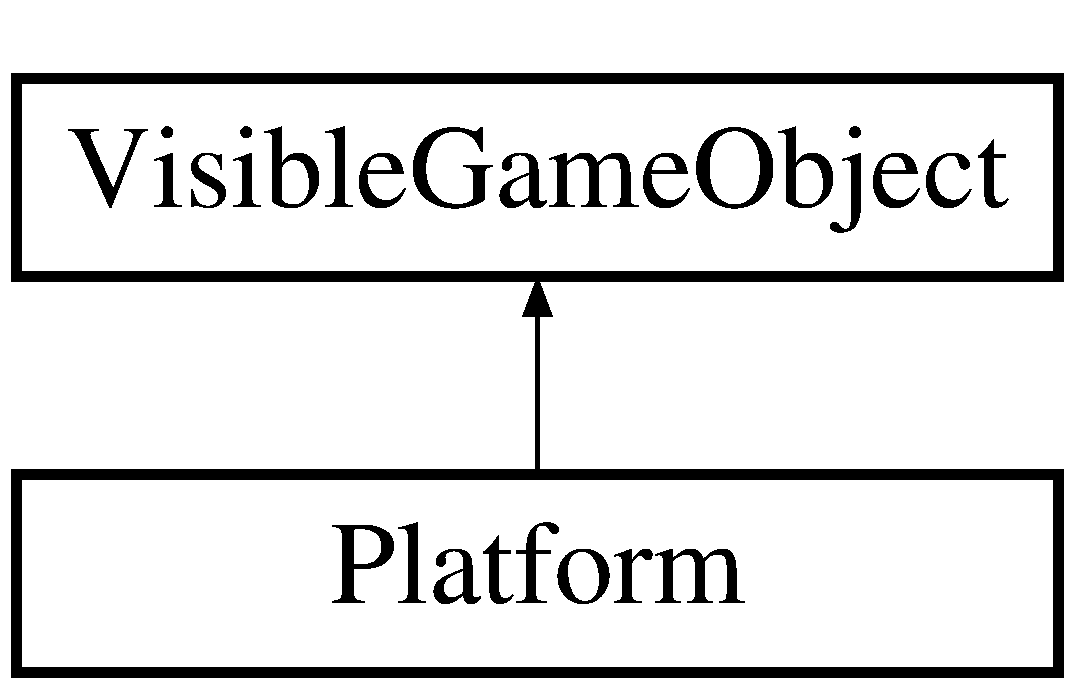
\includegraphics[height=2.000000cm]{classPlatform}
\end{center}
\end{figure}
\subsection*{Public Member Functions}
\begin{DoxyCompactItemize}
\item 
{\bf Platform} (const std\+::string \&f\+Name, sf\+::\+Vector2f size, sf\+::\+Vector2f position)
\begin{DoxyCompactList}\small\item\em Constructor. \end{DoxyCompactList}\item 
{\bf $\sim$\+Platform} ()\label{classPlatform_a13b5e4ef946b8a2fe38d22014145ab68}

\begin{DoxyCompactList}\small\item\em The destructor. \end{DoxyCompactList}\item 
void {\bf Draw} (sf\+::\+Render\+Window \&window)
\begin{DoxyCompactList}\small\item\em Draw this object on the window. \end{DoxyCompactList}\item 
bool {\bf check\+Collision} ({\bf Visible\+Game\+Object} $\ast$other, float e)
\item 
void {\bf Update} (float elapsed\+Time, sf\+::\+Event \&\+\_\+event, std\+::map$<$ std\+::string, {\bf Visible\+Game\+Object} $\ast$ $>$ \&\+\_\+object)
\begin{DoxyCompactList}\small\item\em Update this object according to the new event recorded. \end{DoxyCompactList}\end{DoxyCompactItemize}
\subsection*{Data Fields}
\begin{DoxyCompactItemize}
\item 
{\bf Animation} {\bfseries animation}\label{classPlatform_a604c47591a851175dba66ee5309365f3}

\end{DoxyCompactItemize}
\subsection*{Private Attributes}
\begin{DoxyCompactItemize}
\item 
const float {\bfseries v\+Barrier\+Move\+Dist}\label{classPlatform_ab88822aaf8ec1abe72e7b3279af6d7c2}

\end{DoxyCompactItemize}
\subsection*{Additional Inherited Members}


\subsection{Detailed Description}
This class stores any objects that are not \char`\"{}players\char`\"{} for now. New classes for each object can be added later. Objects are differentiated by their \char`\"{}texture filename\char`\"{}. 

Definition at line 15 of file Platform.\+h.



\subsection{Constructor \& Destructor Documentation}
\index{Platform@{Platform}!Platform@{Platform}}
\index{Platform@{Platform}!Platform@{Platform}}
\subsubsection[{Platform(const std\+::string \&f\+Name, sf\+::\+Vector2f size, sf\+::\+Vector2f position)}]{\setlength{\rightskip}{0pt plus 5cm}Platform\+::\+Platform (
\begin{DoxyParamCaption}
\item[{const std\+::string \&}]{f\+Name, }
\item[{sf\+::\+Vector2f}]{size, }
\item[{sf\+::\+Vector2f}]{position}
\end{DoxyParamCaption}
)}\label{classPlatform_a599a6c86435dd0571b69a444bb5529d8}


Constructor. 


\begin{DoxyParams}{Parameters}
{\em f\+Name} & The texture filename. \\
\hline
{\em size} & The size vector. \\
\hline
{\em position} & The position vector. \\
\hline
\end{DoxyParams}


\subsection{Member Function Documentation}
\index{Platform@{Platform}!check\+Collision@{check\+Collision}}
\index{check\+Collision@{check\+Collision}!Platform@{Platform}}
\subsubsection[{check\+Collision(\+Visible\+Game\+Object $\ast$other, float e)}]{\setlength{\rightskip}{0pt plus 5cm}bool Platform\+::check\+Collision (
\begin{DoxyParamCaption}
\item[{{\bf Visible\+Game\+Object} $\ast$}]{other, }
\item[{float}]{e}
\end{DoxyParamCaption}
)}\label{classPlatform_a69a4876867d533deea05444d6a1db170}
Check collision of this object with other objects. Currently does nothing. 
\begin{DoxyParams}{Parameters}
{\em other} & The object to check collision with. \\
\hline
{\em e} & \char`\"{}\+Elasticity\char`\"{} \\
\hline
\end{DoxyParams}
\begin{DoxyReturn}{Returns}
true if collided, false if not. 
\end{DoxyReturn}
\index{Platform@{Platform}!Draw@{Draw}}
\index{Draw@{Draw}!Platform@{Platform}}
\subsubsection[{Draw(sf\+::\+Render\+Window \&window)}]{\setlength{\rightskip}{0pt plus 5cm}void Platform\+::\+Draw (
\begin{DoxyParamCaption}
\item[{sf\+::\+Render\+Window \&}]{window}
\end{DoxyParamCaption}
)\hspace{0.3cm}{\ttfamily [virtual]}}\label{classPlatform_a7b26c99c06289de6a4199377104fc262}


Draw this object on the window. 


\begin{DoxyParams}{Parameters}
{\em window} & The window to draw this object on. \\
\hline
\end{DoxyParams}


Reimplemented from {\bf Visible\+Game\+Object} \doxyref{}{p.}{classVisibleGameObject_a36c4fb68290282364bb198b9b5c4cd07}.

\index{Platform@{Platform}!Update@{Update}}
\index{Update@{Update}!Platform@{Platform}}
\subsubsection[{Update(float elapsed\+Time, sf\+::\+Event \&\+\_\+event, std\+::map$<$ std\+::string, Visible\+Game\+Object $\ast$ $>$ \&\+\_\+object)}]{\setlength{\rightskip}{0pt plus 5cm}void Platform\+::\+Update (
\begin{DoxyParamCaption}
\item[{float}]{elapsed\+Time, }
\item[{sf\+::\+Event \&}]{\+\_\+event, }
\item[{std\+::map$<$ std\+::string, {\bf Visible\+Game\+Object} $\ast$ $>$ \&}]{\+\_\+object}
\end{DoxyParamCaption}
)\hspace{0.3cm}{\ttfamily [virtual]}}\label{classPlatform_aaf13682e0f809e4e0faf4a545501a9b5}


Update this object according to the new event recorded. 


\begin{DoxyParams}{Parameters}
{\em elapsed\+Time} & Time since last update. \\
\hline
{\em \+\_\+event} & The event that triggered this update. \\
\hline
{\em \+\_\+object} & A container containing other objects that might influence this object\textquotesingle{}s position etc. \\
\hline
\end{DoxyParams}


Reimplemented from {\bf Visible\+Game\+Object} \doxyref{}{p.}{classVisibleGameObject_a2760784b238d38161f5b0bbfa46ba427}.



The documentation for this class was generated from the following file\+:\begin{DoxyCompactItemize}
\item 
Platform.\+h\end{DoxyCompactItemize}

\section{Player Class Reference}
\label{classPlayer}\index{Player@{Player}}


Updates and checks Collision of Fire\+Boy/\+Water\+Girl with various objects.  


Inheritance diagram for Player\+:\begin{figure}[H]
\begin{center}
\leavevmode
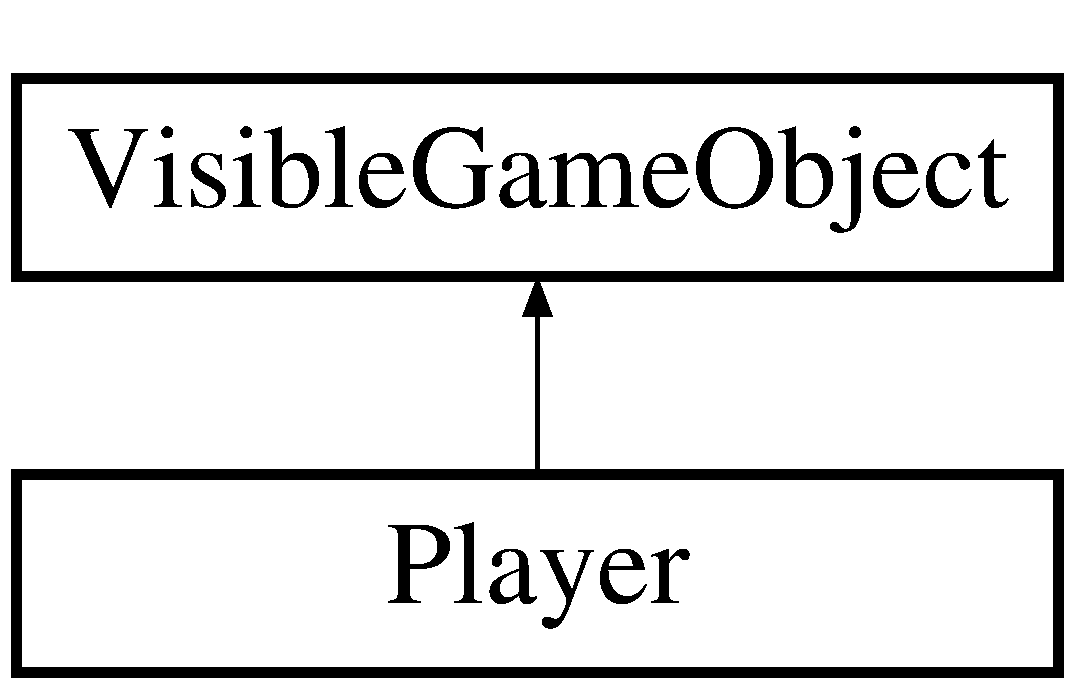
\includegraphics[height=2.000000cm]{classPlayer}
\end{center}
\end{figure}
\subsection*{Public Member Functions}
\begin{DoxyCompactItemize}
\item 
{\bf Player} (const std\+::string \&f\+Name, sf\+::\+Keyboard\+::\+Key \+\_\+u, sf\+::\+Keyboard\+::\+Key \+\_\+l, sf\+::\+Keyboard\+::\+Key \+\_\+r)
\begin{DoxyCompactList}\small\item\em Constructor for player. \end{DoxyCompactList}\item 
void {\bf Update} (float elapsed\+Time, sf\+::\+Event \&\+\_\+event, std\+::map$<$ std\+::string, {\bf Visible\+Game\+Object} $\ast$ $>$ \&\+\_\+object)
\begin{DoxyCompactList}\small\item\em Takes an event as input and updates the player according to it. \end{DoxyCompactList}\item 
bool {\bf check\+Collision} ({\bf Visible\+Game\+Object} $\ast$other, float e)
\begin{DoxyCompactList}\small\item\em Takes an object and checks for collision of player with it. \end{DoxyCompactList}\end{DoxyCompactItemize}
\subsection*{Data Fields}
\begin{DoxyCompactItemize}
\item 
{\bf Animation} {\bf animation}\label{classPlayer_a9f7bf0ea89a4585b3247187409a83efa}

\begin{DoxyCompactList}\small\item\em \doxyref{Animation}{p.}{classAnimation} object which takes care of animation of object. \end{DoxyCompactList}\end{DoxyCompactItemize}
\subsection*{Private Attributes}
\begin{DoxyCompactItemize}
\item 
const float {\bf v\+Barrier\+Move\+Dist}\label{classPlayer_adf055a2b9e01a046d705730500bac25d}

\begin{DoxyCompactList}\small\item\em Distance moved by barrier upon activation by a switch. \end{DoxyCompactList}\item 
sf\+::\+Keyboard\+::\+Key {\bf u}\label{classPlayer_a37696731b6f5f0b03ba02a3e039f52bb}

\begin{DoxyCompactList}\small\item\em Key for upward movement. \end{DoxyCompactList}\item 
sf\+::\+Keyboard\+::\+Key {\bf l}\label{classPlayer_a8a66f34dab6d571b1062fe5745c2f524}

\begin{DoxyCompactList}\small\item\em Key for left movement. \end{DoxyCompactList}\item 
sf\+::\+Keyboard\+::\+Key {\bf r}\label{classPlayer_a67499db9ed2768ecdb3fbc7e5c7135fb}

\begin{DoxyCompactList}\small\item\em Key for right movement. \end{DoxyCompactList}\item 
bool {\bf is\+Up\+Pressed}\label{classPlayer_a80f447e22745905e58126c77fea06ee7}

\begin{DoxyCompactList}\small\item\em Checks if up key is pressed. \end{DoxyCompactList}\item 
bool {\bf is\+L\+Pressed}\label{classPlayer_acbdfbf6f7abe2a0725cdd1aceac5480a}

\begin{DoxyCompactList}\small\item\em Checks if left key is pressed. \end{DoxyCompactList}\item 
bool {\bf is\+R\+Pressed}\label{classPlayer_ab57005b45fdff6ff4e5d4a6fa081ffb1}

\begin{DoxyCompactList}\small\item\em Checks if right key is pressed. \end{DoxyCompactList}\item 
bool {\bf is\+Jumping}\label{classPlayer_aab294bec9f8fed91bb7d599e37bfd5f6}

\begin{DoxyCompactList}\small\item\em is It falling down after ataining max distance it can jump? Not if it is actually jumping \end{DoxyCompactList}\item 
float {\bf d\+Jump}\label{classPlayer_a0d51cb52a9554ea9828febc836c30f79}

\begin{DoxyCompactList}\small\item\em The distance it jumped before falling down. \end{DoxyCompactList}\item 
float {\bf \+\_\+up\+Vel}\label{classPlayer_aec33fb9bc8d9b1eb9f6c0eb71ef899dd}

\begin{DoxyCompactList}\small\item\em Velocity for Jump. \end{DoxyCompactList}\item 
float {\bf \+\_\+x\+Val}\label{classPlayer_a5b5ce3f912d9713076d07edbaa65c554}

\begin{DoxyCompactList}\small\item\em Velocity to move left/right. \end{DoxyCompactList}\item 
float {\bf \+\_\+velocity}\label{classPlayer_a6eead0ba8bf0a30264deeb066f30e9a9}

\begin{DoxyCompactList}\small\item\em Downward Velocity. \end{DoxyCompactList}\item 
float {\bf \+\_\+max\+Velocity}\label{classPlayer_a45568f07b5fe8d9e578e433d69e4b87e}

\begin{DoxyCompactList}\small\item\em Max velocity. \end{DoxyCompactList}\end{DoxyCompactItemize}
\subsection*{Additional Inherited Members}


\subsection{Detailed Description}
Updates and checks Collision of Fire\+Boy/\+Water\+Girl with various objects. 

The player inherits from the \doxyref{Visible\+Game\+Object}{p.}{classVisibleGameObject} class and takes control of the Fireboy and Watergirl\textquotesingle{}s updates. 

Definition at line 12 of file Player.\+h.



\subsection{Constructor \& Destructor Documentation}
\index{Player@{Player}!Player@{Player}}
\index{Player@{Player}!Player@{Player}}
\subsubsection[{Player(const std\+::string \&f\+Name, sf\+::\+Keyboard\+::\+Key \+\_\+u, sf\+::\+Keyboard\+::\+Key \+\_\+l, sf\+::\+Keyboard\+::\+Key \+\_\+r)}]{\setlength{\rightskip}{0pt plus 5cm}Player\+::\+Player (
\begin{DoxyParamCaption}
\item[{const std\+::string \&}]{f\+Name, }
\item[{sf\+::\+Keyboard\+::\+Key}]{\+\_\+u, }
\item[{sf\+::\+Keyboard\+::\+Key}]{\+\_\+l, }
\item[{sf\+::\+Keyboard\+::\+Key}]{\+\_\+r}
\end{DoxyParamCaption}
)}\label{classPlayer_a76ca9e2f31375ea484dc13604bfdd14e}


Constructor for player. 


\begin{DoxyParams}{Parameters}
{\em f\+Name} & File name for loading the texture. \\
\hline
{\em \+\_\+u} & Key for jumping the player \\
\hline
{\em \+\_\+l} & Key for going left. \\
\hline
{\em \+\_\+r} & Key for going right \begin{DoxyVerb} The constructor initialises the members like maximum vecloity attainable by player, max
 jump height and other parameters.

 Sets the animation of the player as well.\end{DoxyVerb}
 \\
\hline
\end{DoxyParams}


\subsection{Member Function Documentation}
\index{Player@{Player}!check\+Collision@{check\+Collision}}
\index{check\+Collision@{check\+Collision}!Player@{Player}}
\subsubsection[{check\+Collision(\+Visible\+Game\+Object $\ast$other, float e)}]{\setlength{\rightskip}{0pt plus 5cm}bool Player\+::check\+Collision (
\begin{DoxyParamCaption}
\item[{{\bf Visible\+Game\+Object} $\ast$}]{other, }
\item[{float}]{e}
\end{DoxyParamCaption}
)}\label{classPlayer_a480331d13e5c4661970aff8cdb70a38a}


Takes an object and checks for collision of player with it. 


\begin{DoxyParams}{Parameters}
{\em other} & \\
\hline
{\em e} & \\
\hline
\end{DoxyParams}
\begin{DoxyReturn}{Returns}
True if collision occured false otherwise. e value checks the elasticity of collosion. If e = 0.\+0 then it pushes the player back and other object stays put. If e = 1 then object moves easily with a push. 
\end{DoxyReturn}
\index{Player@{Player}!Update@{Update}}
\index{Update@{Update}!Player@{Player}}
\subsubsection[{Update(float elapsed\+Time, sf\+::\+Event \&\+\_\+event, std\+::map$<$ std\+::string, Visible\+Game\+Object $\ast$ $>$ \&\+\_\+object)}]{\setlength{\rightskip}{0pt plus 5cm}void Player\+::\+Update (
\begin{DoxyParamCaption}
\item[{float}]{elapsed\+Time, }
\item[{sf\+::\+Event \&}]{\+\_\+event, }
\item[{std\+::map$<$ std\+::string, {\bf Visible\+Game\+Object} $\ast$ $>$ \&}]{\+\_\+object}
\end{DoxyParamCaption}
)\hspace{0.3cm}{\ttfamily [virtual]}}\label{classPlayer_a3e44a2494b4169bd0cc3d3f0f5a9dbd7}


Takes an event as input and updates the player according to it. 


\begin{DoxyParams}{Parameters}
{\em elapsed\+Time} & \\
\hline
{\em \+\_\+event} & \\
\hline
{\em \+\_\+object} & Checks for any events that are trigerred for the player , like going up or going left or right.\\
\hline
\end{DoxyParams}
It checks for collisions also for every player with any object .

Animates the object by giving a Texture to it by the corresponding state of game. 

Reimplemented from {\bf Visible\+Game\+Object} \doxyref{}{p.}{classVisibleGameObject_a2760784b238d38161f5b0bbfa46ba427}.



The documentation for this class was generated from the following file\+:\begin{DoxyCompactItemize}
\item 
Player.\+h\end{DoxyCompactItemize}

\section{Server Class Reference}
\label{classServer}\index{Server@{Server}}


A server over T\+CP to enable networking.  




{\ttfamily \#include $<$Server.\+h$>$}

\subsection*{Public Member Functions}
\begin{DoxyCompactItemize}
\item 
{\bf Server} (unsigned short \+\_\+port1, unsigned short \+\_\+port2)
\begin{DoxyCompactList}\small\item\em The constructor. \end{DoxyCompactList}\item 
void {\bf wait\+For\+Client\+Send\+Socket} (bool $\ast$res)
\begin{DoxyCompactList}\small\item\em Listen to and accept connections from the client at \+\_\+port1. \end{DoxyCompactList}\item 
void {\bf wait\+For\+Client\+Listen\+Socket} (bool $\ast$res)
\begin{DoxyCompactList}\small\item\em Listen to and accept connections from the client at \+\_\+port2. \end{DoxyCompactList}\end{DoxyCompactItemize}
\subsection*{Data Fields}
\begin{DoxyCompactItemize}
\item 
sf\+::\+Tcp\+Socket {\bf send\+Socket}\label{classServer_a7105cc8419a6e5b9f4ef920bbbcef602}

\begin{DoxyCompactList}\small\item\em Tcp\+Socket used by server to send info to the client. \end{DoxyCompactList}\item 
sf\+::\+Tcp\+Socket {\bf listen\+Socket}\label{classServer_a936d5843a7c2608fc578ba5314547468}

\begin{DoxyCompactList}\small\item\em Tcp\+Socket used by server to receive info from the client. \end{DoxyCompactList}\item 
sf\+::\+Tcp\+Listener {\bf listener}\label{classServer_ab9887f2575ed797c9ac0dd43004a6fc8}

\begin{DoxyCompactList}\small\item\em This listens to connections at \+\_\+port1. \end{DoxyCompactList}\item 
sf\+::\+Tcp\+Listener {\bf listener2}\label{classServer_a54bb5c13f9d06d80d438b3ad484b1729}

\begin{DoxyCompactList}\small\item\em This listens to connections at \+\_\+port2. \end{DoxyCompactList}\end{DoxyCompactItemize}
\subsection*{Private Attributes}
\begin{DoxyCompactItemize}
\item 
unsigned short {\bf port1}\label{classServer_a47b2c62bc2a6801bc0ce543cb9b29e15}

\begin{DoxyCompactList}\small\item\em Port for send\+Socket. \end{DoxyCompactList}\item 
unsigned short {\bf port2}\label{classServer_a1377fadd5460fb552d35e6b53d27d95d}

\begin{DoxyCompactList}\small\item\em Port for listen\+Socket. \end{DoxyCompactList}\end{DoxyCompactItemize}


\subsection{Detailed Description}
A server over T\+CP to enable networking. 

Contains information regarding the network connection with another \char`\"{}\+Client\char`\"{} 

Definition at line 17 of file Server.\+h.



\subsection{Constructor \& Destructor Documentation}
\index{Server@{Server}!Server@{Server}}
\index{Server@{Server}!Server@{Server}}
\subsubsection[{Server(unsigned short \+\_\+port1, unsigned short \+\_\+port2)}]{\setlength{\rightskip}{0pt plus 5cm}Server\+::\+Server (
\begin{DoxyParamCaption}
\item[{unsigned short}]{\+\_\+port1, }
\item[{unsigned short}]{\+\_\+port2}
\end{DoxyParamCaption}
)}\label{classServer_acc86b5037757b339c0ac376a9e67a41d}


The constructor. 


\begin{DoxyParams}{Parameters}
{\em \+\_\+port1} & The port used by this to send info to the client. \\
\hline
{\em \+\_\+port2} & The port used by this to receive info from the client. \\
\hline
\end{DoxyParams}


\subsection{Member Function Documentation}
\index{Server@{Server}!wait\+For\+Client\+Listen\+Socket@{wait\+For\+Client\+Listen\+Socket}}
\index{wait\+For\+Client\+Listen\+Socket@{wait\+For\+Client\+Listen\+Socket}!Server@{Server}}
\subsubsection[{wait\+For\+Client\+Listen\+Socket(bool $\ast$res)}]{\setlength{\rightskip}{0pt plus 5cm}void Server\+::wait\+For\+Client\+Listen\+Socket (
\begin{DoxyParamCaption}
\item[{bool $\ast$}]{res}
\end{DoxyParamCaption}
)}\label{classServer_a52a661ae149028bfbc2d3083ba5ba215}


Listen to and accept connections from the client at \+\_\+port2. 


\begin{DoxyParams}{Parameters}
{\em res} & Store the success/failure of this function in this location. \\
\hline
\end{DoxyParams}
\index{Server@{Server}!wait\+For\+Client\+Send\+Socket@{wait\+For\+Client\+Send\+Socket}}
\index{wait\+For\+Client\+Send\+Socket@{wait\+For\+Client\+Send\+Socket}!Server@{Server}}
\subsubsection[{wait\+For\+Client\+Send\+Socket(bool $\ast$res)}]{\setlength{\rightskip}{0pt plus 5cm}void Server\+::wait\+For\+Client\+Send\+Socket (
\begin{DoxyParamCaption}
\item[{bool $\ast$}]{res}
\end{DoxyParamCaption}
)}\label{classServer_a371c61f93ae66dac9e90cca9594ef323}


Listen to and accept connections from the client at \+\_\+port1. 


\begin{DoxyParams}{Parameters}
{\em res} & Store the success/failure of this function in this location. \\
\hline
\end{DoxyParams}


The documentation for this class was generated from the following file\+:\begin{DoxyCompactItemize}
\item 
Server.\+h\end{DoxyCompactItemize}

\section{Splash Class Reference}
\label{classSplash}\index{Splash@{Splash}}


Saves \doxyref{Game}{p.}{classGame} state.  




{\ttfamily \#include $<$Splash.\+h$>$}

\subsection*{Public Member Functions}
\begin{DoxyCompactItemize}
\item 
int {\bf show} (sf\+::\+Render\+Window \&render\+Window)\label{classSplash_ad1611dd696443a2fd52b30edbe1e857b}

\begin{DoxyCompactList}\small\item\em loads and renders \doxyref{Splash}{p.}{classSplash} Window and splash sprite \end{DoxyCompactList}\end{DoxyCompactItemize}


\subsection{Detailed Description}
Saves \doxyref{Game}{p.}{classGame} state. 

Definition at line 10 of file Splash.\+h.



The documentation for this class was generated from the following file\+:\begin{DoxyCompactItemize}
\item 
Splash.\+h\end{DoxyCompactItemize}

\section{Visible\+Game\+Object Class Reference}
\label{classVisibleGameObject}\index{Visible\+Game\+Object@{Visible\+Game\+Object}}


This class is used to define an object that is to be drawn on the screen.  




{\ttfamily \#include $<$Visible\+Game\+Object.\+h$>$}

Inheritance diagram for Visible\+Game\+Object\+:\begin{figure}[H]
\begin{center}
\leavevmode
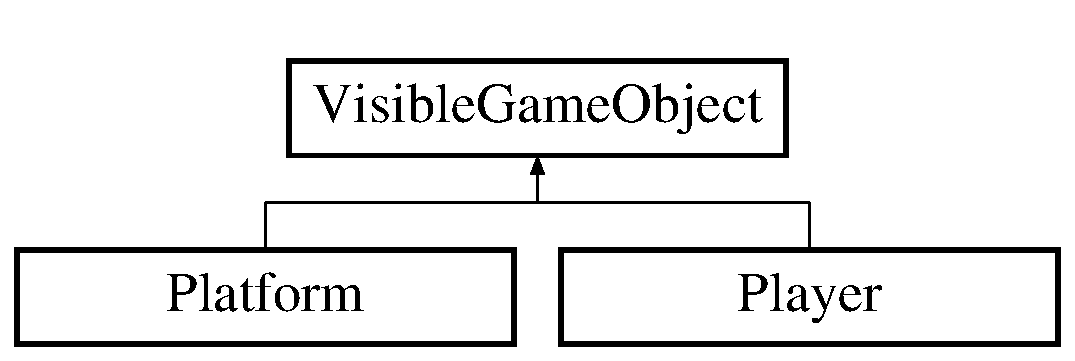
\includegraphics[height=2.000000cm]{classVisibleGameObject}
\end{center}
\end{figure}
\subsection*{Public Types}
\begin{DoxyCompactItemize}
\item 
enum {\bfseries state\+Of\+Obj} \{ \\*
{\bfseries D\+EF}, 
{\bfseries V\+B\+S\+P\+R\+E\+S\+S\+E\+D\+\_\+F}, 
{\bfseries V\+B\+S\+P\+R\+E\+S\+S\+E\+D\+\_\+W}, 
{\bfseries V\+B\+M\+O\+V\+ED}, 
\\*
{\bfseries G\+E\+M\+C\+O\+N\+S\+U\+M\+ED}
 \}\label{classVisibleGameObject_aeea1504090be269d46ca97837a212211}

\end{DoxyCompactItemize}
\subsection*{Public Member Functions}
\begin{DoxyCompactItemize}
\item 
{\bf Visible\+Game\+Object} ()
\begin{DoxyCompactList}\small\item\em The Constructor. \end{DoxyCompactList}\item 
virtual void {\bf Load} (std\+::string filename, float x, float y)
\begin{DoxyCompactList}\small\item\em Load the texture corresponding to the filename. \end{DoxyCompactList}\item 
virtual void {\bf Draw} (sf\+::\+Render\+Window \&window)
\begin{DoxyCompactList}\small\item\em Draw this object on the window. \end{DoxyCompactList}\item 
virtual void {\bf Set\+Position} (float x, float y)
\begin{DoxyCompactList}\small\item\em Set\textquotesingle{}s this object\textquotesingle{}s position, relative to the origin. \end{DoxyCompactList}\item 
virtual void {\bf Update} (float elapsed\+Time, sf\+::\+Event \&event, std\+::map$<$ std\+::string, {\bf Visible\+Game\+Object} $\ast$ $>$ \&\+\_\+object)
\begin{DoxyCompactList}\small\item\em Updates the objects position and texture of the object. \end{DoxyCompactList}\item 
virtual sf\+::\+Vector2f {\bf Get\+Position} () const 
\begin{DoxyCompactList}\small\item\em Get the position of this object. \end{DoxyCompactList}\item 
virtual bool {\bf Is\+Loaded} () const 
\begin{DoxyCompactList}\small\item\em Check the value of \+\_\+is\+Loaded. \end{DoxyCompactList}\item 
virtual sf\+::\+Vector2f {\bf Get\+Half\+Size} ()
\begin{DoxyCompactList}\small\item\em The size vector of the object, divided by 2. \end{DoxyCompactList}\item 
virtual void {\bf move} (float dx, float dy)
\item 
virtual std\+::string {\bf get\+File\+Name} () const 
\begin{DoxyCompactList}\small\item\em Get the file-\/name of the texture for this object. \end{DoxyCompactList}\end{DoxyCompactItemize}
\subsection*{Data Fields}
\begin{DoxyCompactItemize}
\item 
sf\+::\+Rectangle\+Shape {\bf \+\_\+player}\label{classVisibleGameObject_ac9969444fbf1d4dead1bd42ac3b296ef}

\begin{DoxyCompactList}\small\item\em A rectangle shape that is drawable and holds the objects information. \end{DoxyCompactList}\item 
std\+::string {\bf \+\_\+filename}\label{classVisibleGameObject_aa2d1ee273f70eb3994cb411e55b588b9}

\begin{DoxyCompactList}\small\item\em A variable storing the texture\textquotesingle{}s filepath. \end{DoxyCompactList}\item 
state\+Of\+Obj {\bf \+\_\+state\+Of\+Obj}\label{classVisibleGameObject_aba42aaa13e5798b265ce32e0d9192115}

\begin{DoxyCompactList}\small\item\em Stores the state of this object. \end{DoxyCompactList}\end{DoxyCompactItemize}
\subsection*{Protected Attributes}
\begin{DoxyCompactItemize}
\item 
sf\+::\+Texture {\bf player\+Texture}\label{classVisibleGameObject_a9d40b5879eb9b5e2a85be633d022e680}

\begin{DoxyCompactList}\small\item\em Stores the player\textquotesingle{}s texture. \end{DoxyCompactList}\item 
bool {\bf \+\_\+is\+Loaded}\label{classVisibleGameObject_a0276aacb6b6d2c91d2a24a10281d0192}

\begin{DoxyCompactList}\small\item\em Stores whether the texture file was loaded properly. \end{DoxyCompactList}\end{DoxyCompactItemize}


\subsection{Detailed Description}
This class is used to define an object that is to be drawn on the screen. 

All the \doxyref{Game}{p.}{classGame}\textquotesingle{}s Drawable objects must inherit from this class. Currently, most of the type of object checking is done from the object\textquotesingle{}s texture filename. 

Definition at line 13 of file Visible\+Game\+Object.\+h.



\subsection{Constructor \& Destructor Documentation}
\index{Visible\+Game\+Object@{Visible\+Game\+Object}!Visible\+Game\+Object@{Visible\+Game\+Object}}
\index{Visible\+Game\+Object@{Visible\+Game\+Object}!Visible\+Game\+Object@{Visible\+Game\+Object}}
\subsubsection[{Visible\+Game\+Object()}]{\setlength{\rightskip}{0pt plus 5cm}Visible\+Game\+Object\+::\+Visible\+Game\+Object (
\begin{DoxyParamCaption}
{}
\end{DoxyParamCaption}
)}\label{classVisibleGameObject_aa3fcdc2bcf67a8b37398cea587f49df0}


The Constructor. 

Initializes the variabls is\+Loaded and \+\_\+state\+Of\+Obj. 

\subsection{Member Function Documentation}
\index{Visible\+Game\+Object@{Visible\+Game\+Object}!Draw@{Draw}}
\index{Draw@{Draw}!Visible\+Game\+Object@{Visible\+Game\+Object}}
\subsubsection[{Draw(sf\+::\+Render\+Window \&window)}]{\setlength{\rightskip}{0pt plus 5cm}virtual void Visible\+Game\+Object\+::\+Draw (
\begin{DoxyParamCaption}
\item[{sf\+::\+Render\+Window \&}]{window}
\end{DoxyParamCaption}
)\hspace{0.3cm}{\ttfamily [virtual]}}\label{classVisibleGameObject_a36c4fb68290282364bb198b9b5c4cd07}


Draw this object on the window. 


\begin{DoxyParams}{Parameters}
{\em window} & The window to draw this object on. \\
\hline
\end{DoxyParams}


Reimplemented in {\bf Platform} \doxyref{}{p.}{classPlatform_a7b26c99c06289de6a4199377104fc262}.

\index{Visible\+Game\+Object@{Visible\+Game\+Object}!get\+File\+Name@{get\+File\+Name}}
\index{get\+File\+Name@{get\+File\+Name}!Visible\+Game\+Object@{Visible\+Game\+Object}}
\subsubsection[{get\+File\+Name() const }]{\setlength{\rightskip}{0pt plus 5cm}virtual std\+::string Visible\+Game\+Object\+::get\+File\+Name (
\begin{DoxyParamCaption}
{}
\end{DoxyParamCaption}
) const\hspace{0.3cm}{\ttfamily [virtual]}}\label{classVisibleGameObject_a5d42ab296f524880889d7b70811bcf15}


Get the file-\/name of the texture for this object. 

\begin{DoxyReturn}{Returns}
A string containing the filepath (relative to the source directory) 
\end{DoxyReturn}
\index{Visible\+Game\+Object@{Visible\+Game\+Object}!Get\+Half\+Size@{Get\+Half\+Size}}
\index{Get\+Half\+Size@{Get\+Half\+Size}!Visible\+Game\+Object@{Visible\+Game\+Object}}
\subsubsection[{Get\+Half\+Size()}]{\setlength{\rightskip}{0pt plus 5cm}virtual sf\+::\+Vector2f Visible\+Game\+Object\+::\+Get\+Half\+Size (
\begin{DoxyParamCaption}
{}
\end{DoxyParamCaption}
)\hspace{0.3cm}{\ttfamily [inline]}, {\ttfamily [virtual]}}\label{classVisibleGameObject_a656a7f68be590c95888cacef26e7465e}


The size vector of the object, divided by 2. 

\begin{DoxyReturn}{Returns}
A vector\+: (size.\+x/2, size.\+y/2) 
\end{DoxyReturn}


Definition at line 68 of file Visible\+Game\+Object.\+h.



References \+\_\+player.

\index{Visible\+Game\+Object@{Visible\+Game\+Object}!Get\+Position@{Get\+Position}}
\index{Get\+Position@{Get\+Position}!Visible\+Game\+Object@{Visible\+Game\+Object}}
\subsubsection[{Get\+Position() const }]{\setlength{\rightskip}{0pt plus 5cm}virtual sf\+::\+Vector2f Visible\+Game\+Object\+::\+Get\+Position (
\begin{DoxyParamCaption}
{}
\end{DoxyParamCaption}
) const\hspace{0.3cm}{\ttfamily [virtual]}}\label{classVisibleGameObject_a5c8b63273d977475d2dc1f337d2e52d0}


Get the position of this object. 

\begin{DoxyReturn}{Returns}
A float vector representing this object\textquotesingle{}s position. 
\end{DoxyReturn}
\index{Visible\+Game\+Object@{Visible\+Game\+Object}!Is\+Loaded@{Is\+Loaded}}
\index{Is\+Loaded@{Is\+Loaded}!Visible\+Game\+Object@{Visible\+Game\+Object}}
\subsubsection[{Is\+Loaded() const }]{\setlength{\rightskip}{0pt plus 5cm}virtual bool Visible\+Game\+Object\+::\+Is\+Loaded (
\begin{DoxyParamCaption}
{}
\end{DoxyParamCaption}
) const\hspace{0.3cm}{\ttfamily [virtual]}}\label{classVisibleGameObject_a025faedc39b9292a9a8a9a1c5763f3a9}


Check the value of \+\_\+is\+Loaded. 

\begin{DoxyReturn}{Returns}
true if the texture file has been loaded properly, false otherwise 
\end{DoxyReturn}
\index{Visible\+Game\+Object@{Visible\+Game\+Object}!Load@{Load}}
\index{Load@{Load}!Visible\+Game\+Object@{Visible\+Game\+Object}}
\subsubsection[{Load(std\+::string filename, float x, float y)}]{\setlength{\rightskip}{0pt plus 5cm}virtual void Visible\+Game\+Object\+::\+Load (
\begin{DoxyParamCaption}
\item[{std\+::string}]{filename, }
\item[{float}]{x, }
\item[{float}]{y}
\end{DoxyParamCaption}
)\hspace{0.3cm}{\ttfamily [virtual]}}\label{classVisibleGameObject_a1977aa9f59f00a2e4bdd9b494d0b7899}


Load the texture corresponding to the filename. 


\begin{DoxyParams}{Parameters}
{\em filename} & The location of this object\textquotesingle{}s texture file. \\
\hline
{\em x} & The x size (width) of the this object \\
\hline
{\em y} & The y size (height) of this object \\
\hline
\end{DoxyParams}
\index{Visible\+Game\+Object@{Visible\+Game\+Object}!move@{move}}
\index{move@{move}!Visible\+Game\+Object@{Visible\+Game\+Object}}
\subsubsection[{move(float dx, float dy)}]{\setlength{\rightskip}{0pt plus 5cm}virtual void Visible\+Game\+Object\+::move (
\begin{DoxyParamCaption}
\item[{float}]{dx, }
\item[{float}]{dy}
\end{DoxyParamCaption}
)\hspace{0.3cm}{\ttfamily [inline]}, {\ttfamily [virtual]}}\label{classVisibleGameObject_a7e39ff4808f601732abe7eb638fdfc83}
Moves the player by the corresponding offsets. 
\begin{DoxyParams}{Parameters}
{\em dx} & The displacement in X direction. \\
\hline
{\em dy} & The displacement in Y direction. \\
\hline
\end{DoxyParams}


Definition at line 74 of file Visible\+Game\+Object.\+h.



References \+\_\+player.

\index{Visible\+Game\+Object@{Visible\+Game\+Object}!Set\+Position@{Set\+Position}}
\index{Set\+Position@{Set\+Position}!Visible\+Game\+Object@{Visible\+Game\+Object}}
\subsubsection[{Set\+Position(float x, float y)}]{\setlength{\rightskip}{0pt plus 5cm}virtual void Visible\+Game\+Object\+::\+Set\+Position (
\begin{DoxyParamCaption}
\item[{float}]{x, }
\item[{float}]{y}
\end{DoxyParamCaption}
)\hspace{0.3cm}{\ttfamily [virtual]}}\label{classVisibleGameObject_a1a3c4566e9ee101b3d57bf64f6881211}


Set\textquotesingle{}s this object\textquotesingle{}s position, relative to the origin. 


\begin{DoxyParams}{Parameters}
{\em x} & X-\/\+Coodinate of the position. \\
\hline
{\em y} & Y-\/\+Coodinate of the position. \\
\hline
\end{DoxyParams}
\index{Visible\+Game\+Object@{Visible\+Game\+Object}!Update@{Update}}
\index{Update@{Update}!Visible\+Game\+Object@{Visible\+Game\+Object}}
\subsubsection[{Update(float elapsed\+Time, sf\+::\+Event \&event, std\+::map$<$ std\+::string, Visible\+Game\+Object $\ast$ $>$ \&\+\_\+object)}]{\setlength{\rightskip}{0pt plus 5cm}virtual void Visible\+Game\+Object\+::\+Update (
\begin{DoxyParamCaption}
\item[{float}]{elapsed\+Time, }
\item[{sf\+::\+Event \&}]{event, }
\item[{std\+::map$<$ std\+::string, {\bf Visible\+Game\+Object} $\ast$ $>$ \&}]{\+\_\+object}
\end{DoxyParamCaption}
)\hspace{0.3cm}{\ttfamily [virtual]}}\label{classVisibleGameObject_a2760784b238d38161f5b0bbfa46ba427}


Updates the objects position and texture of the object. 


\begin{DoxyParams}{Parameters}
{\em elapsed\+Time} & The time elapsed since last update (sort of simulates frame rate) \\
\hline
{\em event} & The event that occured. \\
\hline
{\em \+\_\+object} & A map of all other objects to be drawn.\\
\hline
\end{DoxyParams}
Checks the \+\_\+object map to update this object according to the position of other objects in game. An example is checking for collisions. 

Reimplemented in {\bf Platform} \doxyref{}{p.}{classPlatform_aaf13682e0f809e4e0faf4a545501a9b5}, and {\bf Player} \doxyref{}{p.}{classPlayer_a3e44a2494b4169bd0cc3d3f0f5a9dbd7}.



The documentation for this class was generated from the following file\+:\begin{DoxyCompactItemize}
\item 
Visible\+Game\+Object.\+h\end{DoxyCompactItemize}

%--- End generated contents ---

% Index
\backmatter
\newpage
\phantomsection
\clearemptydoublepage
\addcontentsline{toc}{chapter}{Index}
\printindex

\end{document}
